\usepackage{graphicx}


\newcommand{\latency}{
    \begin{figure}[!t]
    \centering
    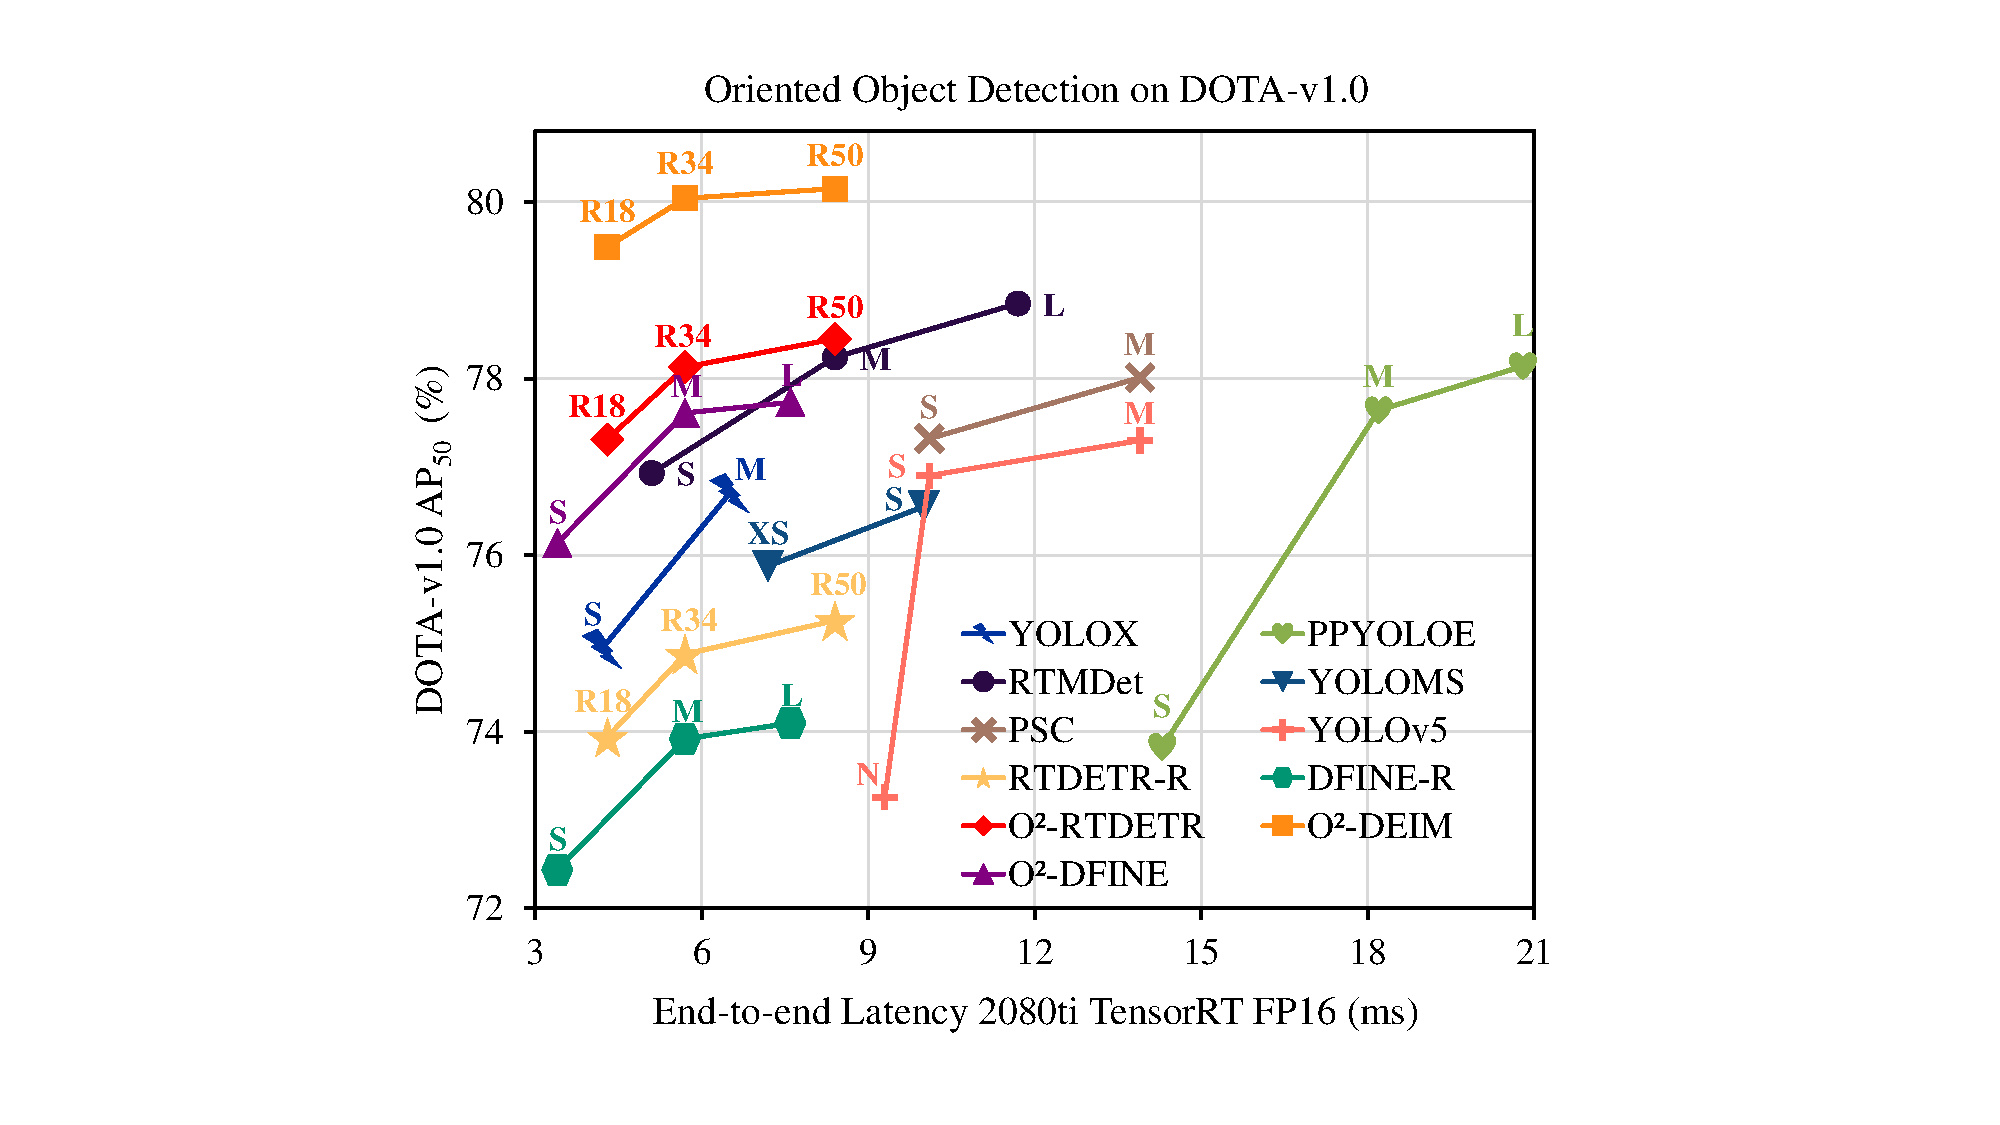
\includegraphics[width=0.95\linewidth]{latency.pdf}
    \caption{Compared to existing real-time object detectors, the family of O$^2$-DFINE, O$^2$-RTDETR, and O$^2$-DEIM achieves competitive performance.}
    \label{latency}
    \end{figure}

}


\newcommand{\differentConfThre}{
    \begin{figure}[!t]
    \centering
    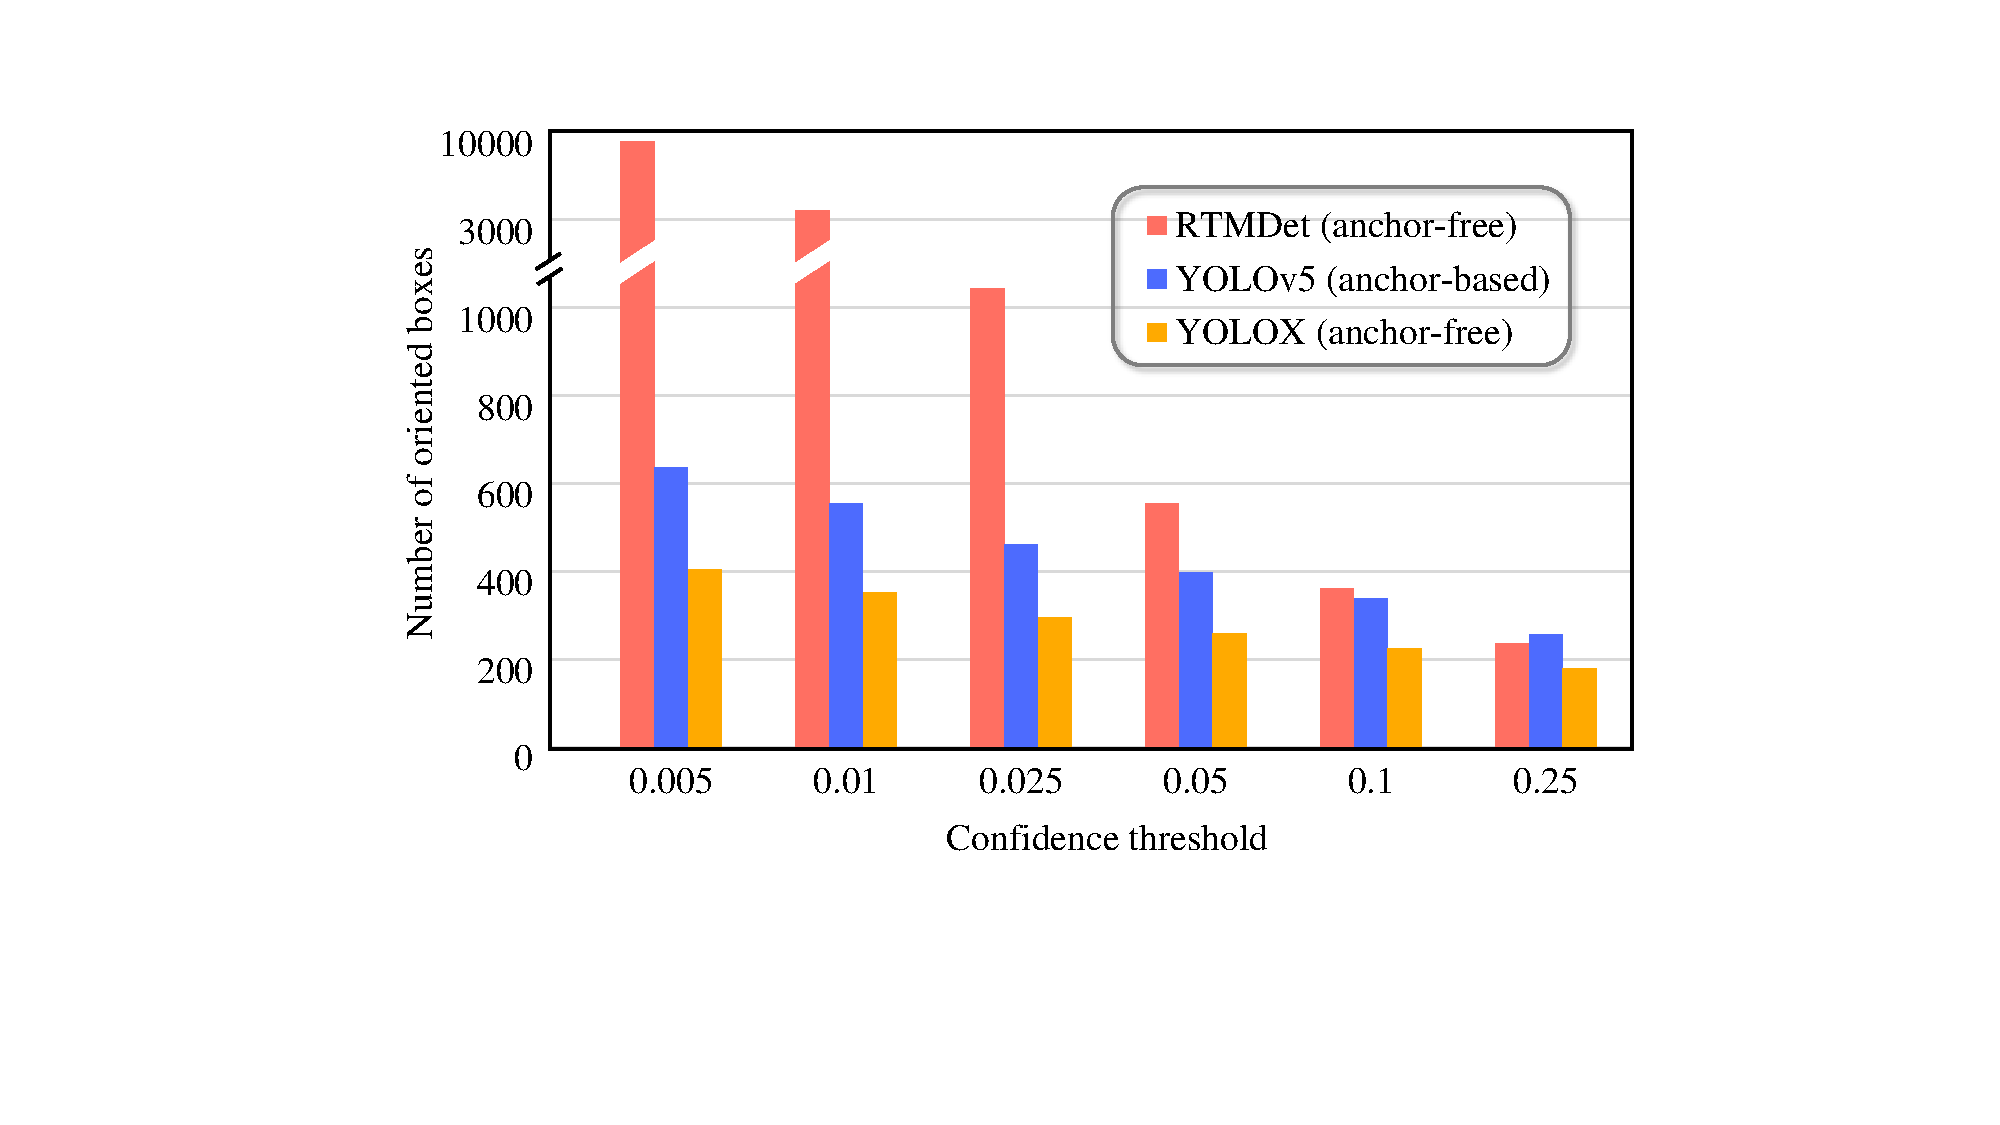
\includegraphics[width=0.95\linewidth]{different_conf_thre.pdf}
    \caption{The number of remaining oriented boxes above different confidence thresholds in rotated NMS.}
    \label{differentConfThre}
    \vspace{-0.5em}
    \end{figure}
}

\newcommand{\NMSExeTime}{
    \begin{figure}[!t]
    \centering
    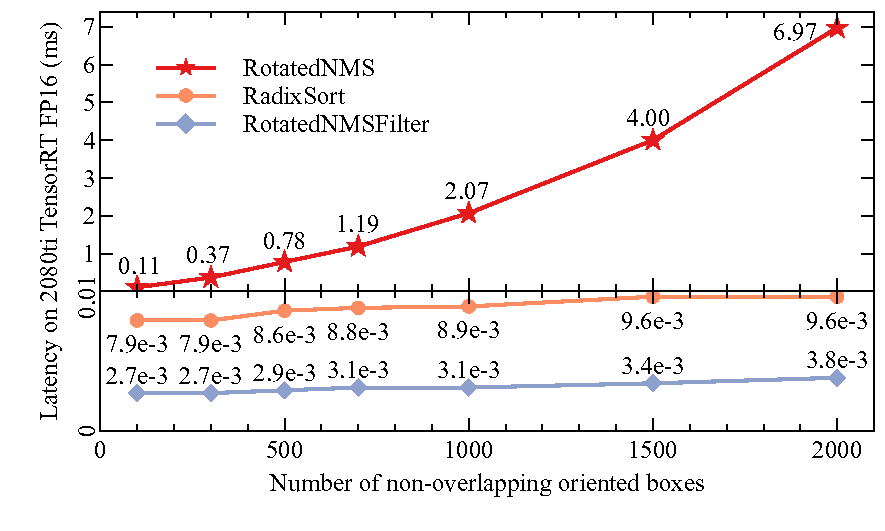
\includegraphics[width=0.95\linewidth]{rotated_nms_exe_time.pdf}
    \caption{Execution time of rotated NMS with different numbers of non-overlapping oriented boxes on the 2080ti (TensorRT FP16).}
    \label{NMSExeTime}
    \vspace{-0.5em}
    \end{figure}
}

\newcommand{\angleDistribution}{
    \begin{figure*}[!t]
    \centering
    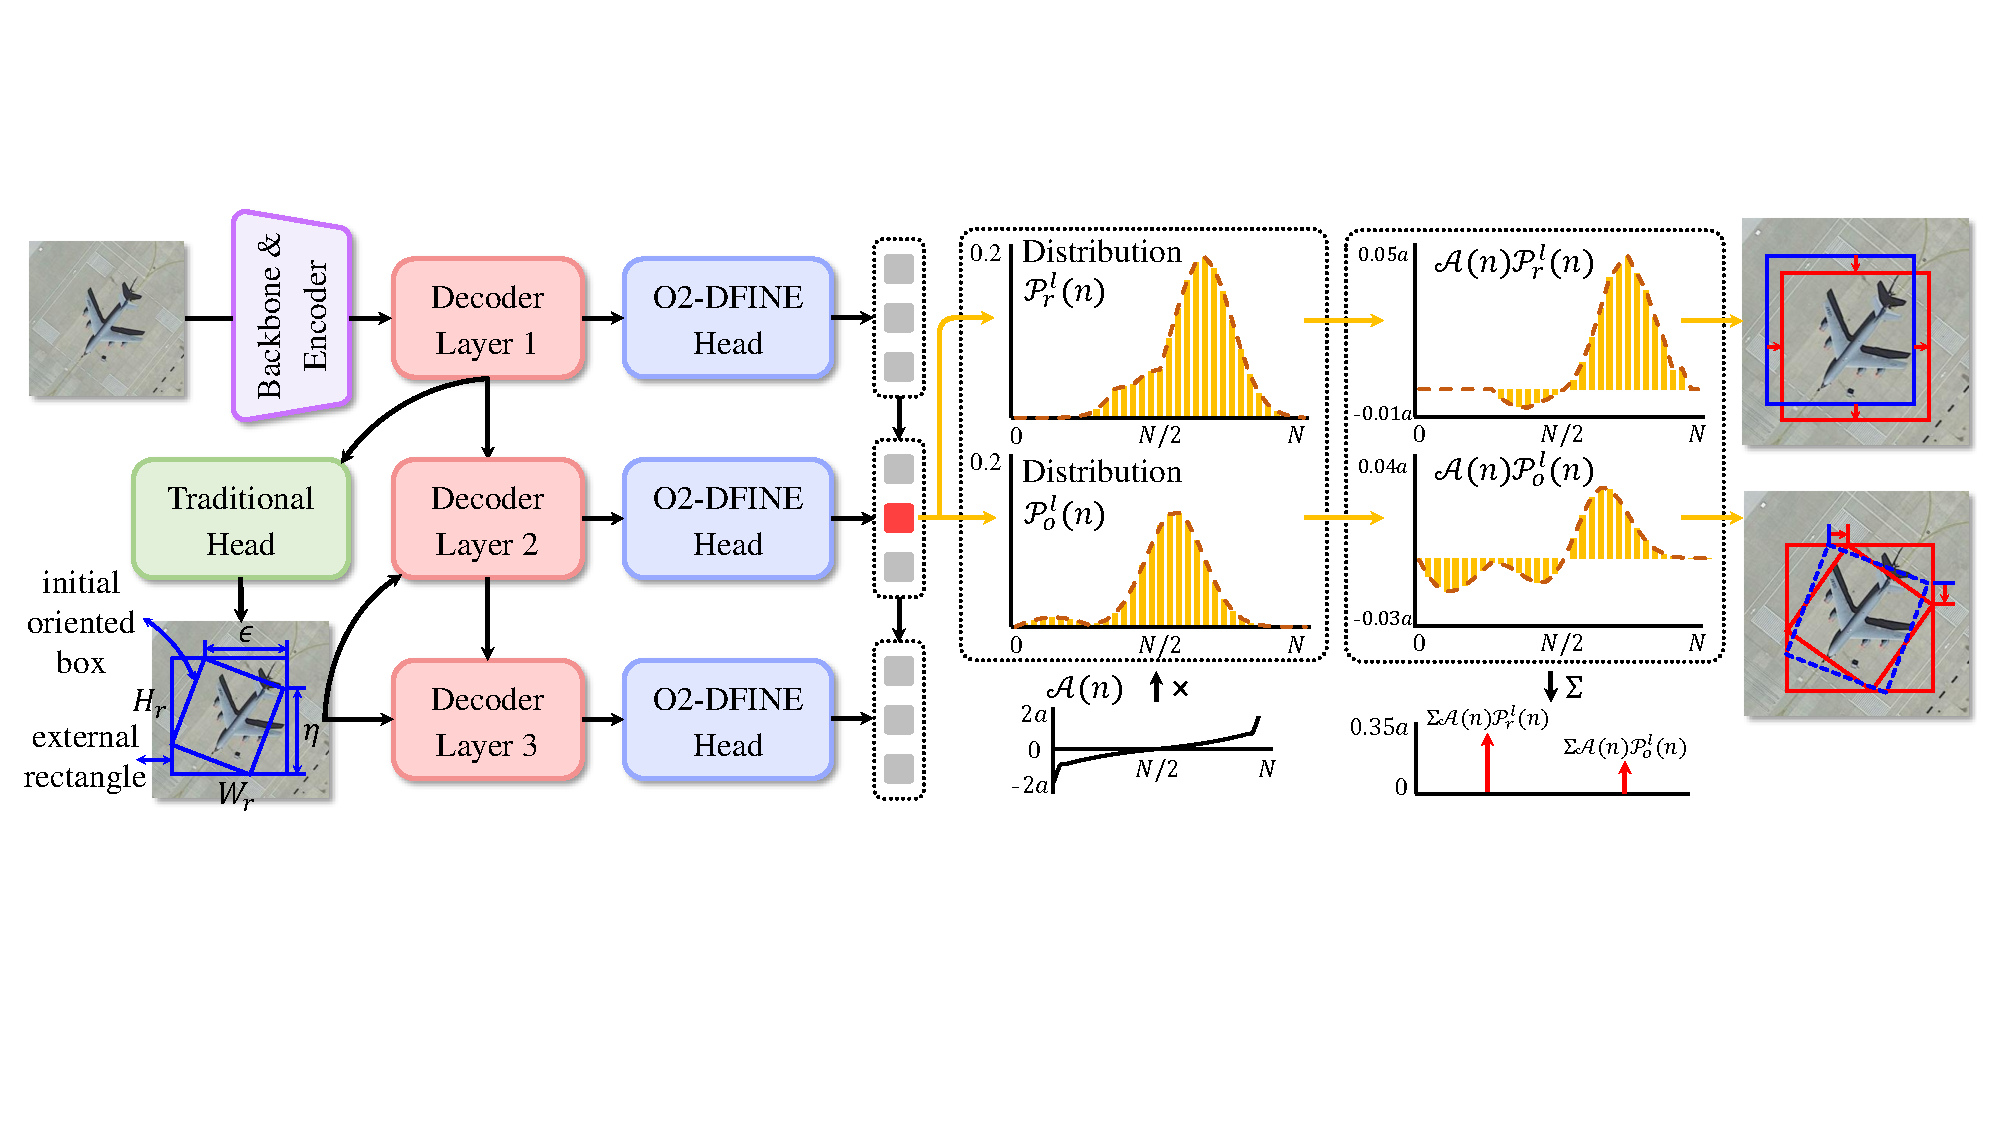
\includegraphics[width=\linewidth]{angle_distribution.pdf}
    \caption{Overview of O$^2$-DFINE with Angle Distribution Refinement. Oriented boxes are learned in a decoupled manner using probability distributions as fine-grained representations of the external rectangle and vertex offsets, which are iteratively refined across decoder layers in a residual fashion.}
    \label{angleDistribution}
    \vspace{-1em}
    \end{figure*}
}

\newcommand{\charmferDistance}{
    \begin{figure*}[!t]
    \centering
    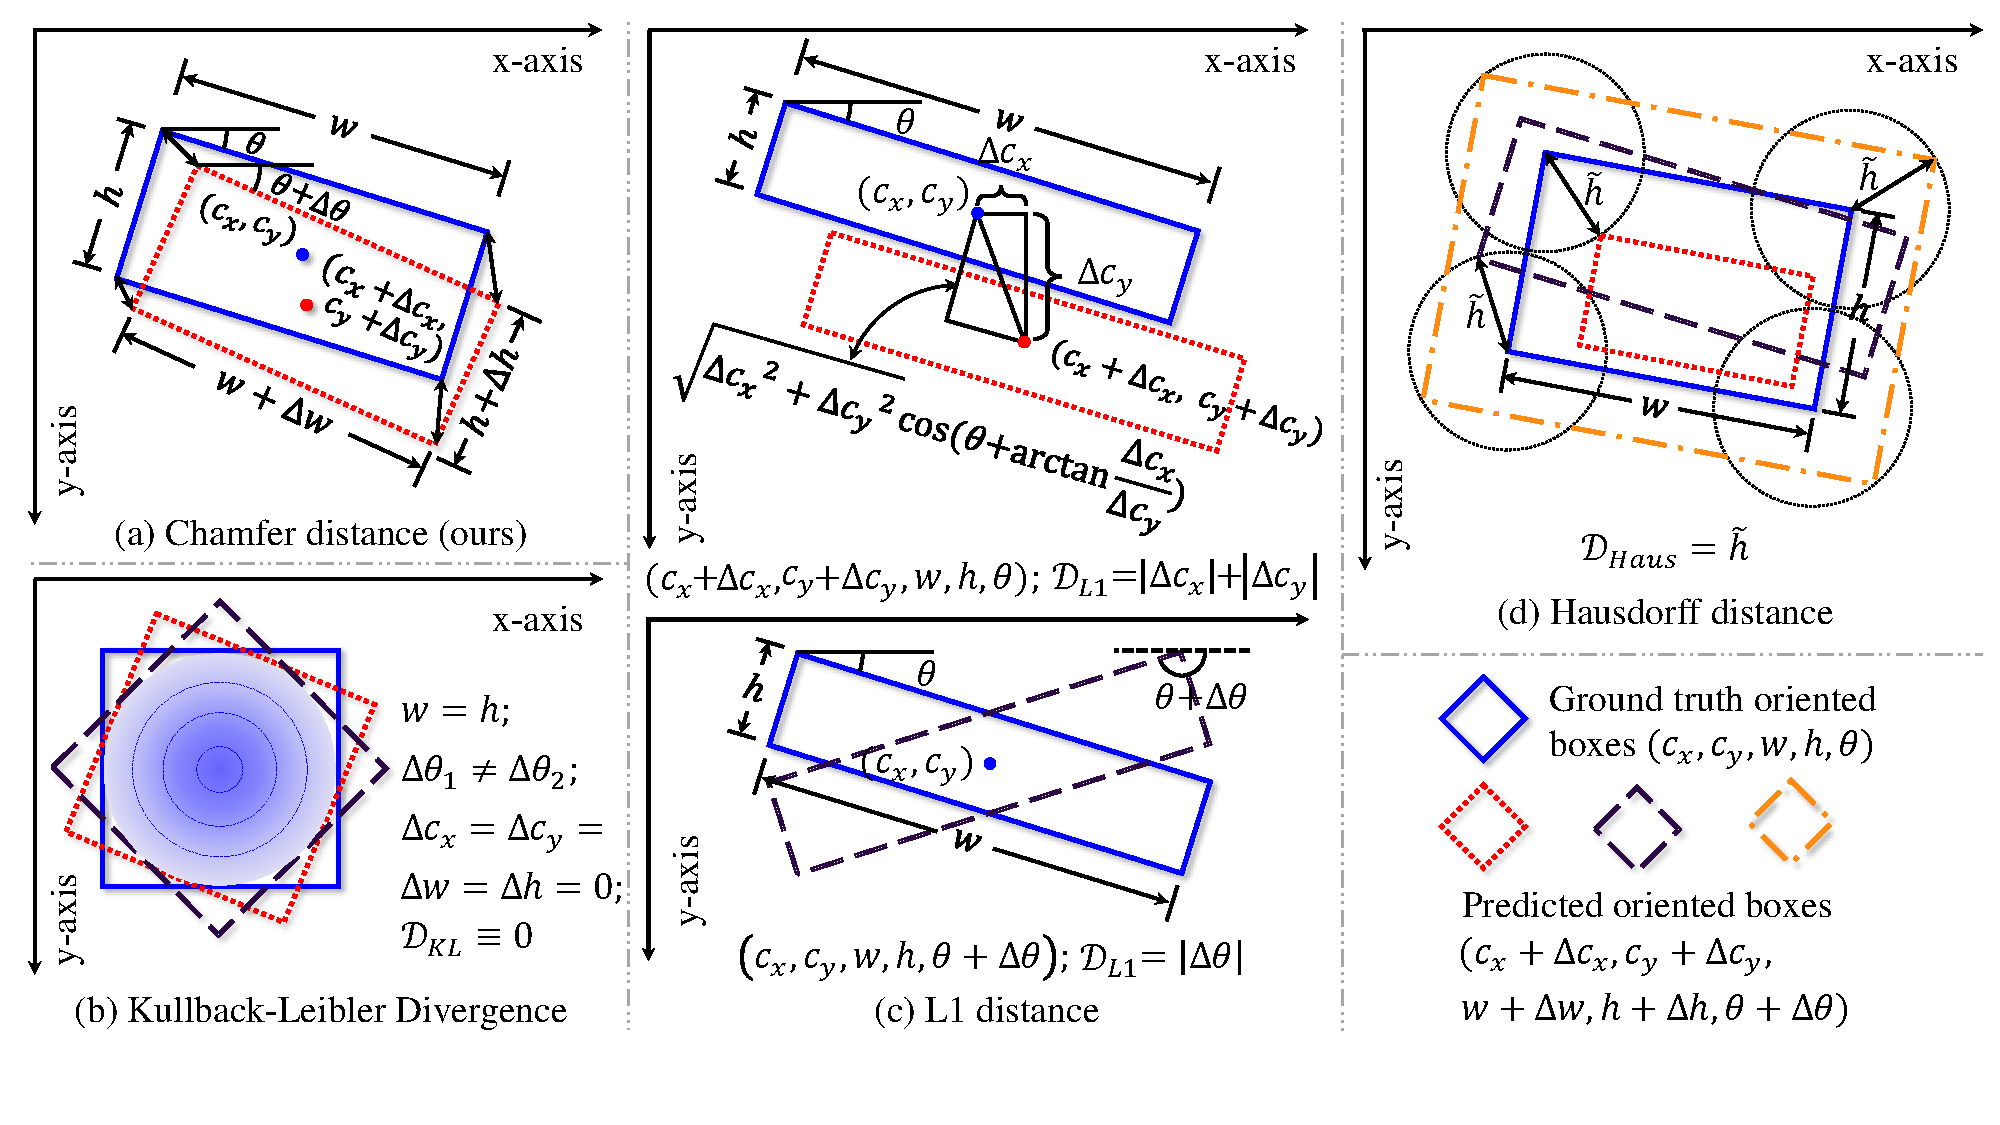
\includegraphics[width=0.95\linewidth]{chamfer_distance_cost.pdf}
    \caption{Distance cost for bipartite matching. (a) Chamfer distance (ours). (b) Kullback-Leibler Divergence. (c)  L1 distance. (d) Hausdorff distance.}
    \label{charmferDistance}
    \vspace{-0.5em}
    \end{figure*}
}


\newcommand{\contrastiveDenoise}{
    \begin{figure*}[!t]
    \centering
    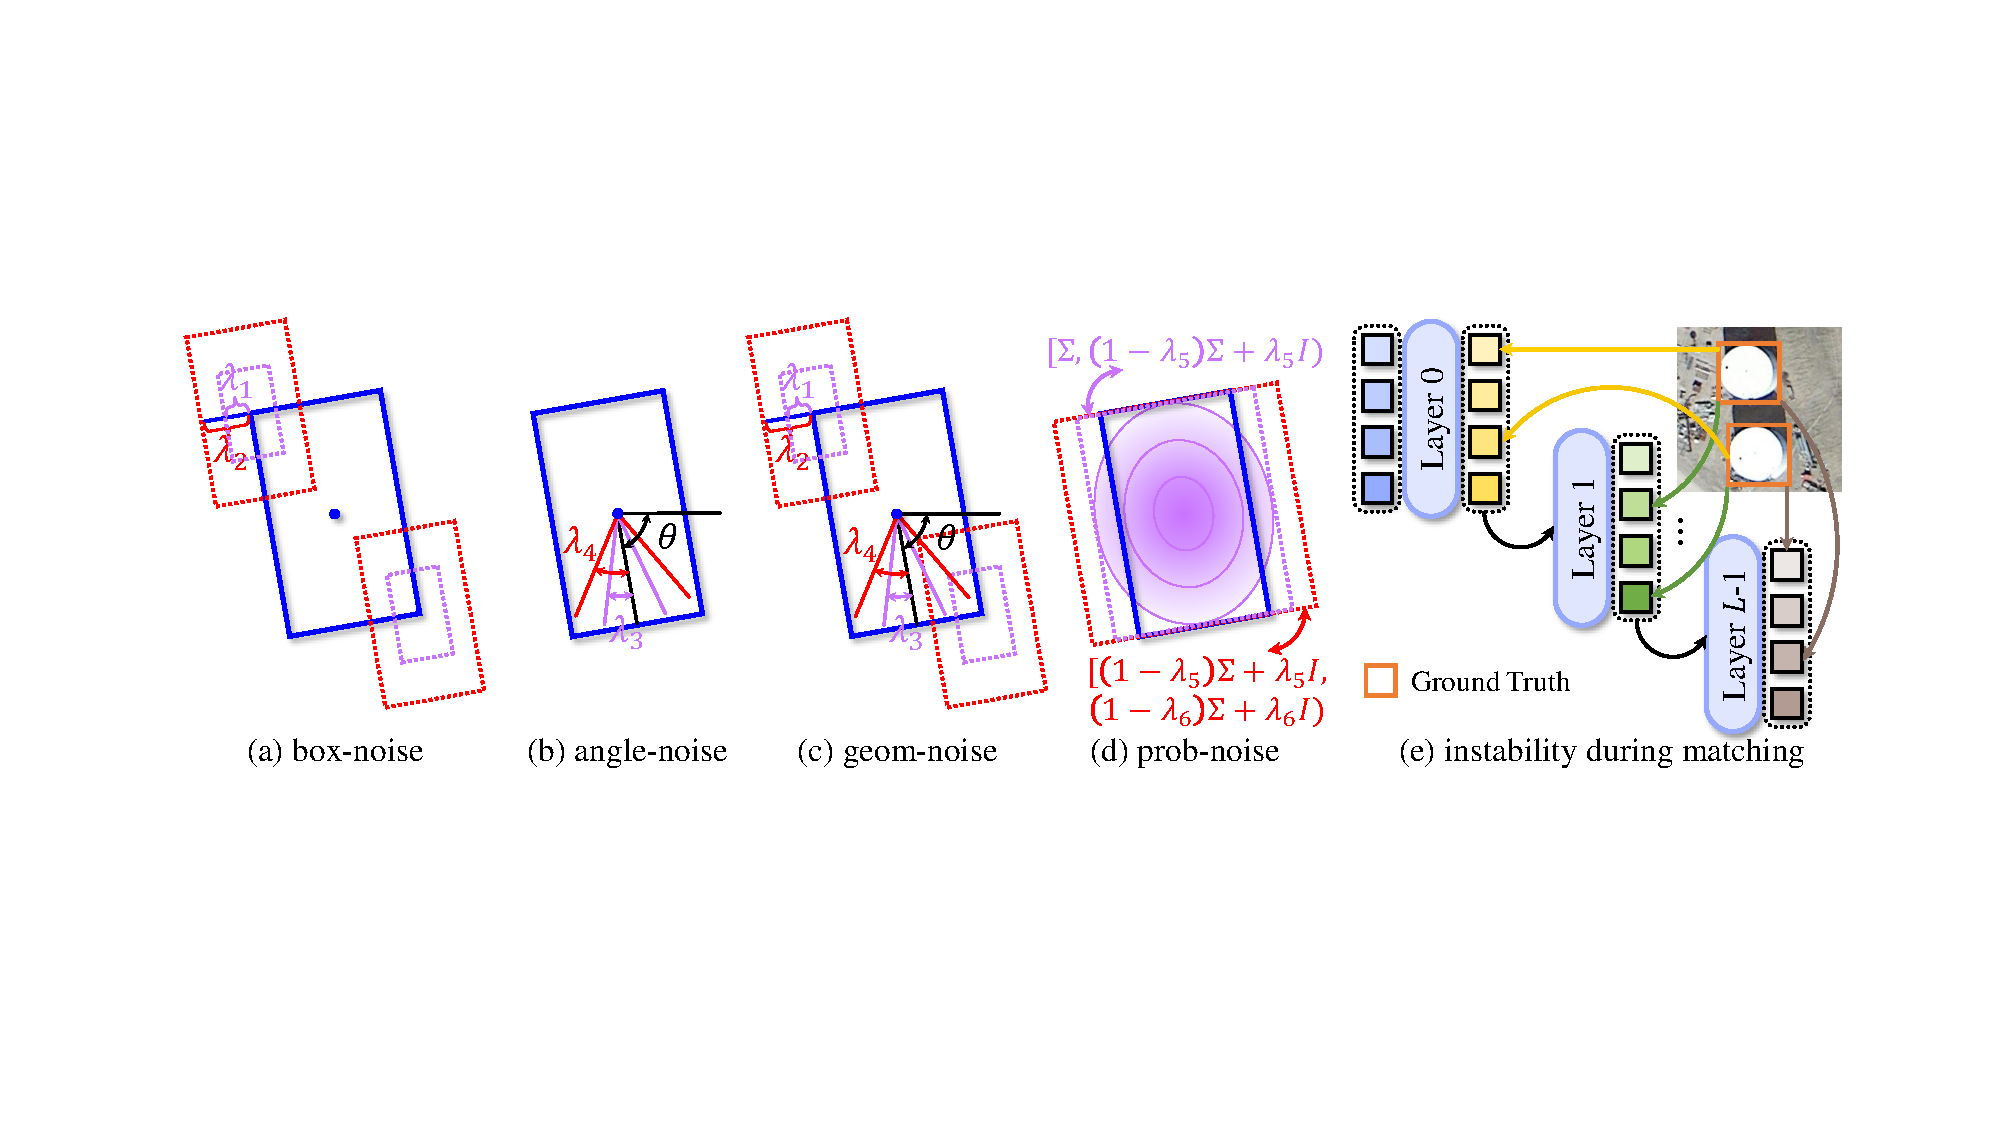
\includegraphics[width=\linewidth]{contrastive_denoising.pdf}
    \caption{Oriented Contrastive Denoising. (a) Box noise. (b) Angle noise. (c) Geometric noise. (d) Probability noise. (e) Instability during mathcing.}
    \label{contrastiveDenoise}
    \vspace{-0.5em}
    \end{figure*}
}

\newcommand{\instability}{
    \begin{figure}[!t]
    \centering
    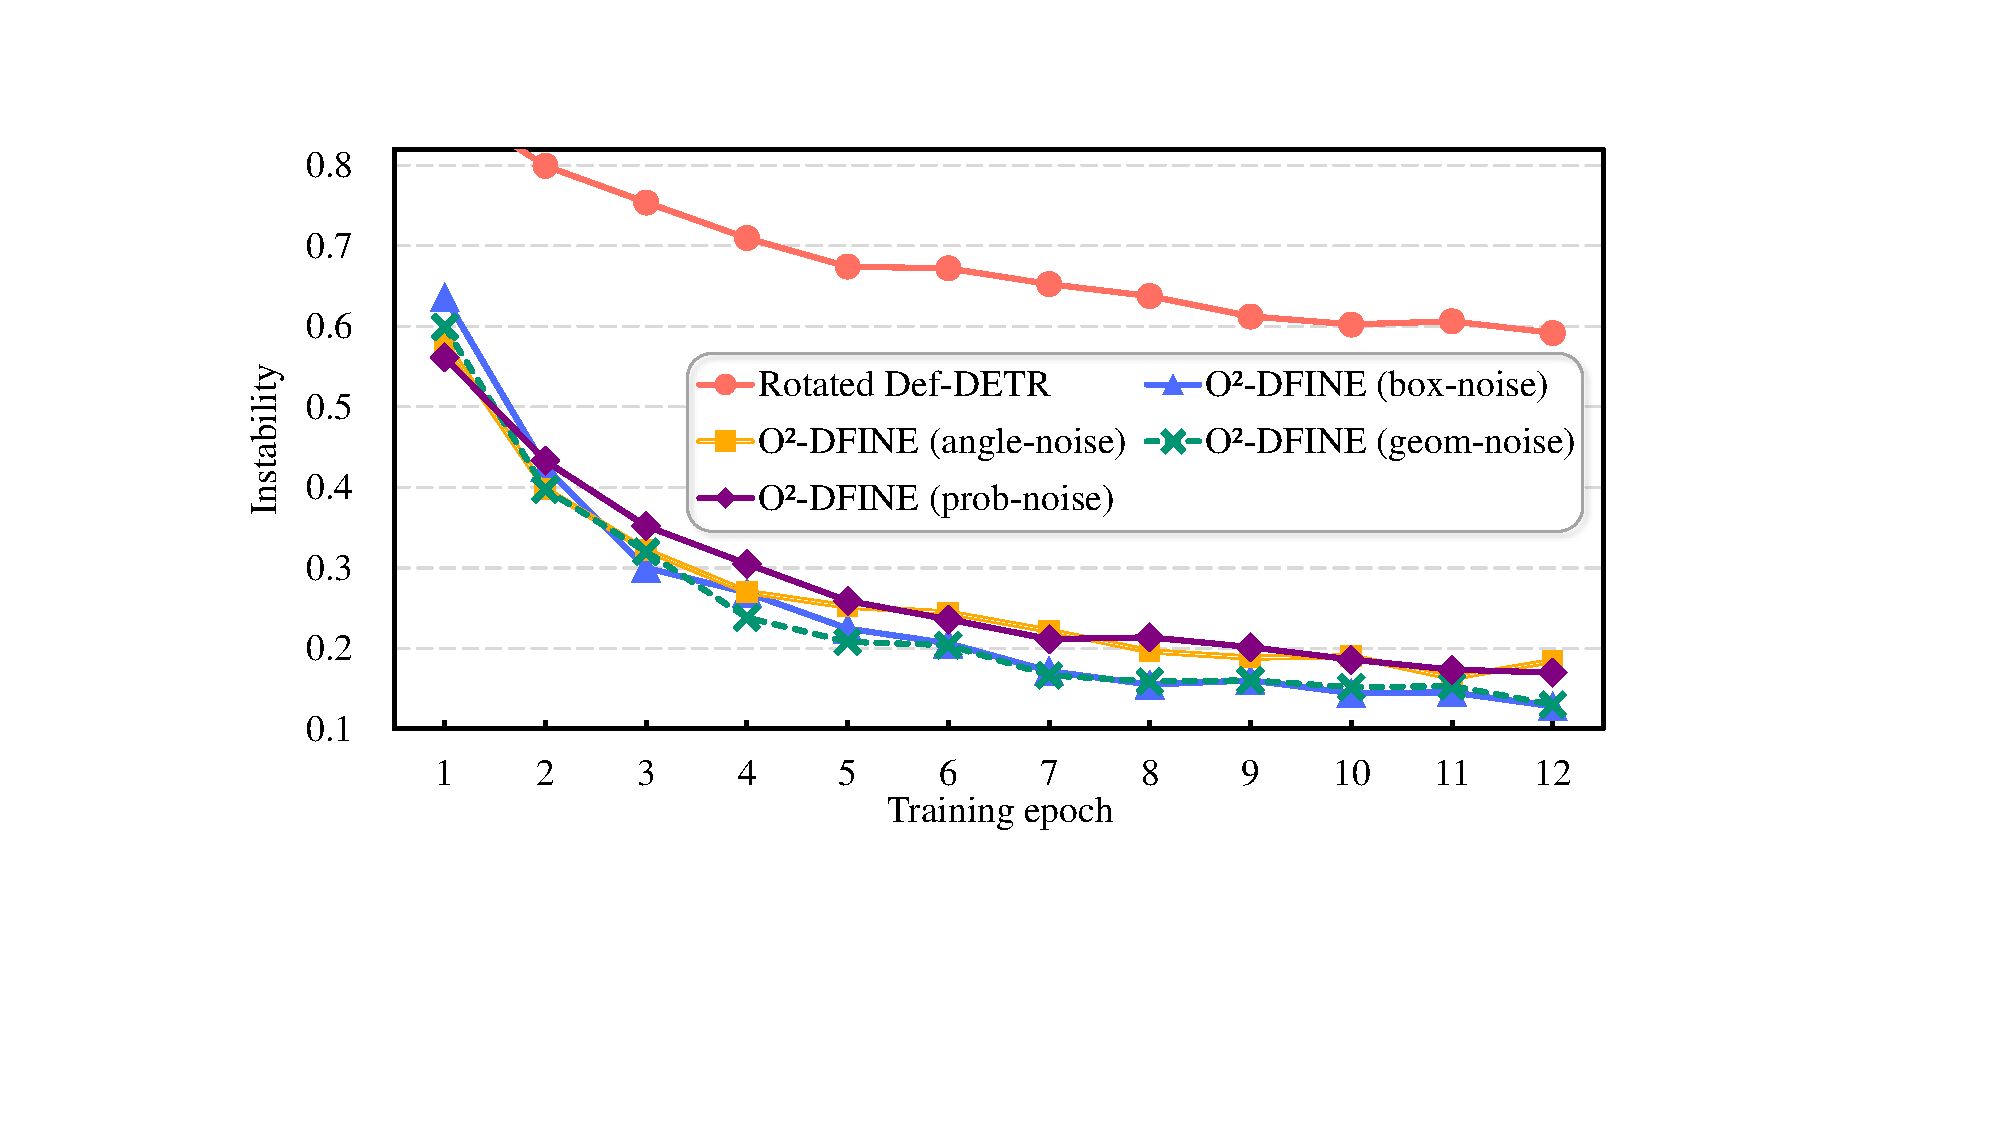
\includegraphics[width=0.95\linewidth]{instability.pdf}
    \caption{The instability metric of Oriented Contrastive Denoising.}
    \label{instability}
    \end{figure}
}


\definecolor{mypurple}{RGB}{202, 115, 255}


\newcommand{\visualContrastiveDenoise}{
    \begin{figure}[t]
      \centering
       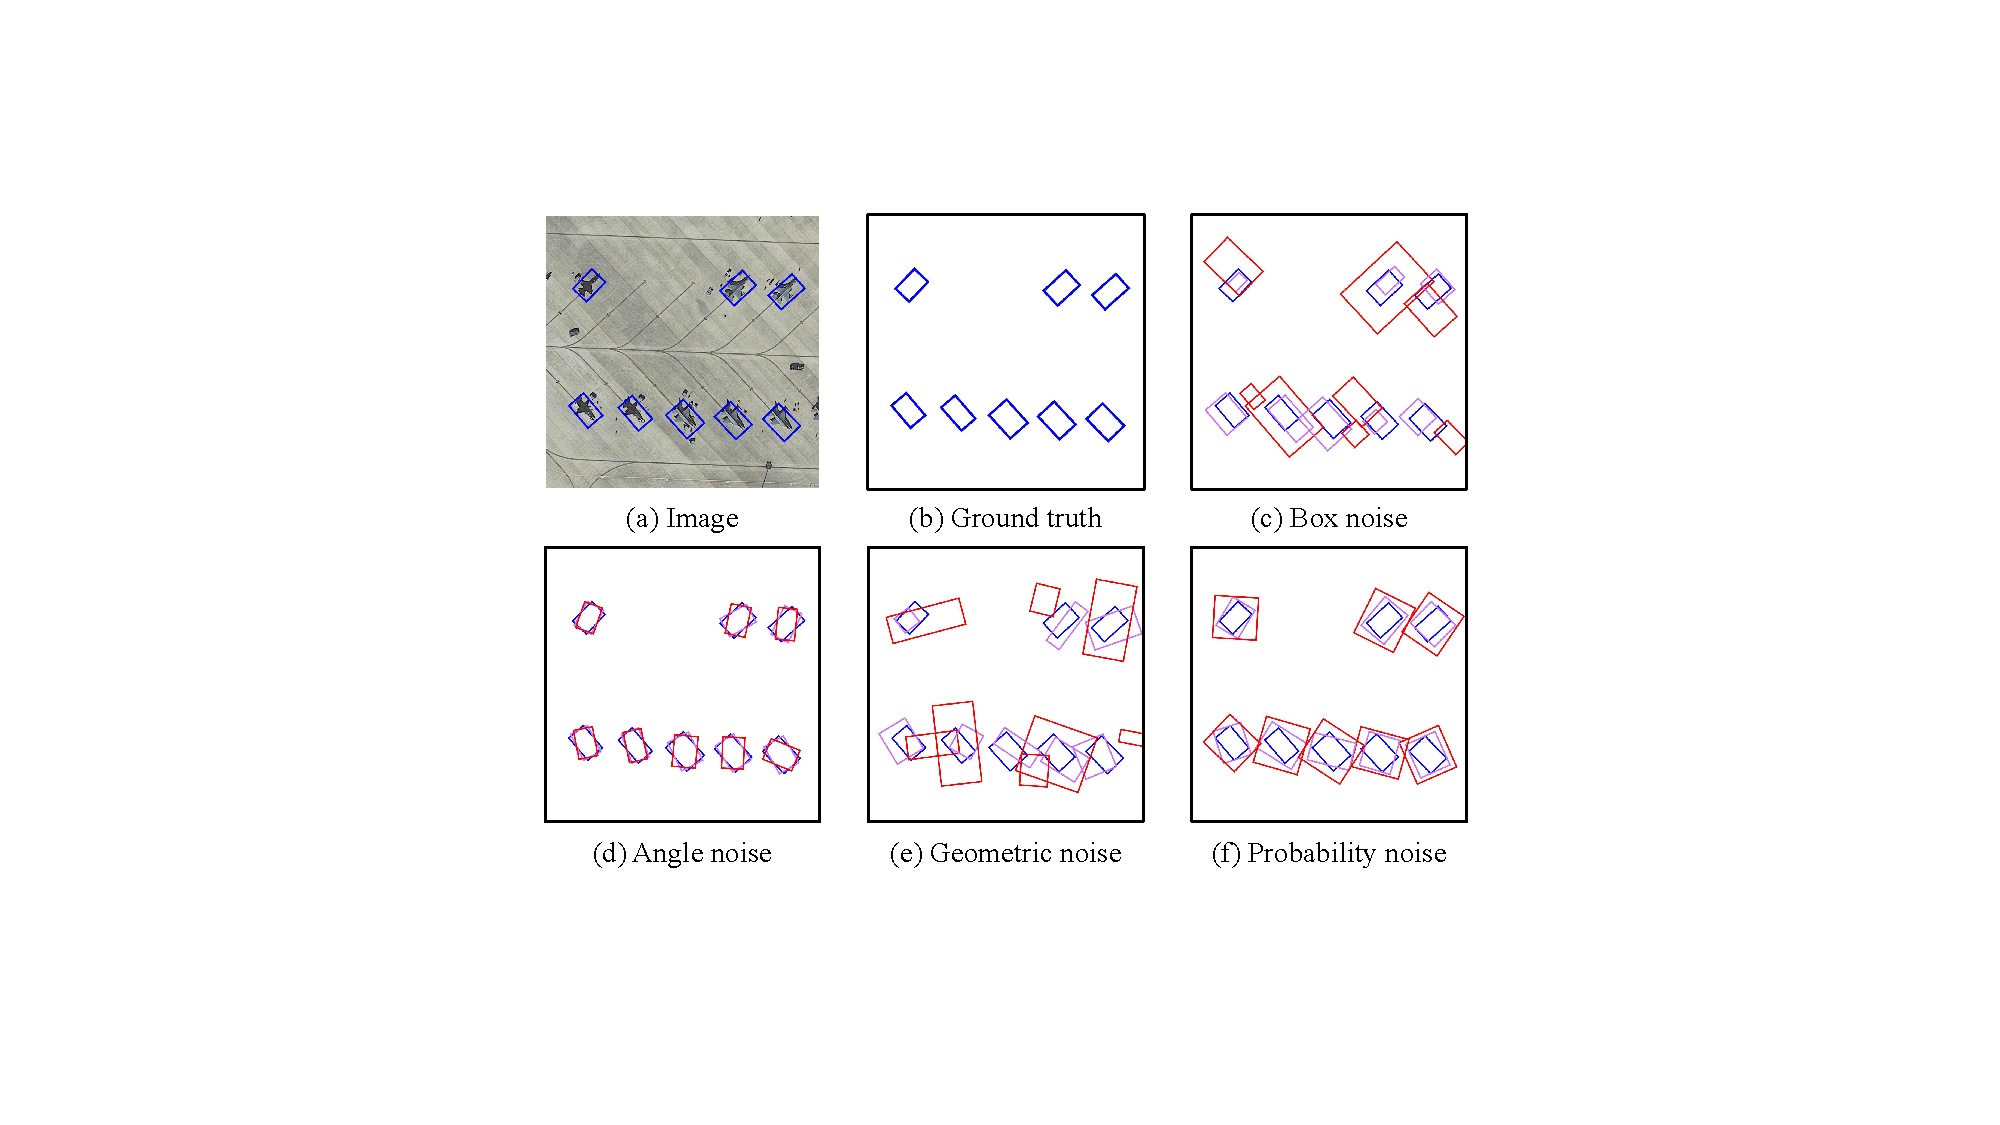
\includegraphics[width=0.95\linewidth]{visual_contrastive_denoising.pdf}
        \parbox{0.75\linewidth}{\footnotesize
          \raisebox{-1ex}{\rotatebox{45}{\tikz{\draw[blue, thick] (0,0) rectangle (2ex,2ex);}}} ground truth \hfill
          \raisebox{-1ex}{\rotatebox{45}{\tikz{\draw[mypurple, thick] (0,0) rectangle (2ex,2ex);}}} positive \hfill
          \raisebox{-1ex}{\rotatebox{45}{\tikz{\draw[red, thick] (0,0) rectangle (2ex,2ex);}}} negtive
          %\textcolor{blue}{$\blacksquare$} ground truth \hfill
          %\textcolor{mypurple}{$\blacksquare$} positive \hfill
          %\textcolor{red}{$\blacksquare$} negtive \hfill
        }
       \caption{Qualitative analysis of Oriented Contrastive Denoising. (a) An image example. (b) Ground-truth oriented boxes. (c) The box noise. (d) The angle noise. (e) The geometric noise. (f) The probability noise example.}
       \label{visual_contrastive_denoising}
    \end{figure}
}



\newcommand{\heatmap}{
    \begin{figure}[t]
      \centering
       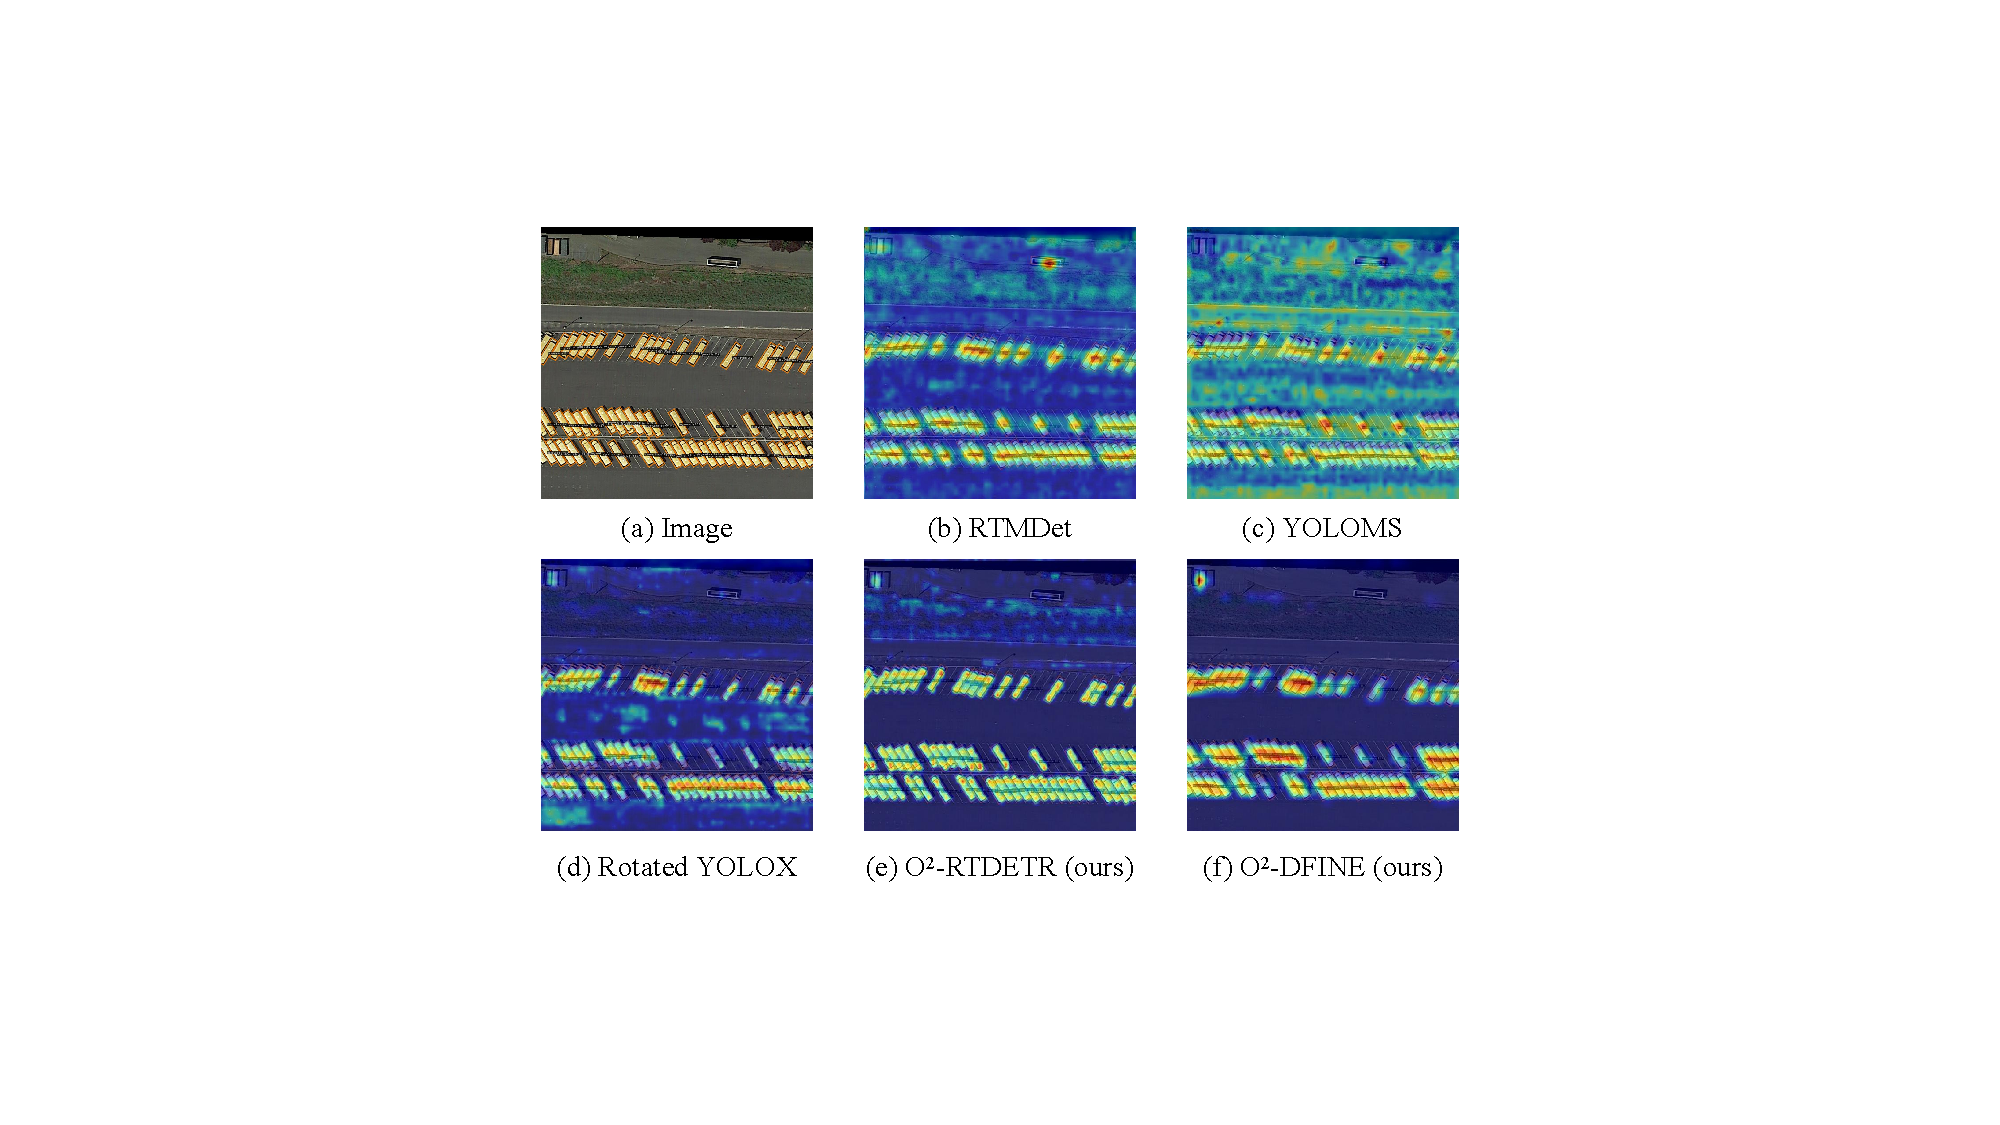
\includegraphics[width=0.95\linewidth]{heatmap.pdf}
       \caption{Visualization of backbone output feature maps. The heatmaps show that our method yields more concentrated and object-aligned activations compared to other methods.}
       \label{visual_heatmap}
    \end{figure}
}

\newcommand{\visualChamfer}{
\begin{figure}[t]
  \centering
       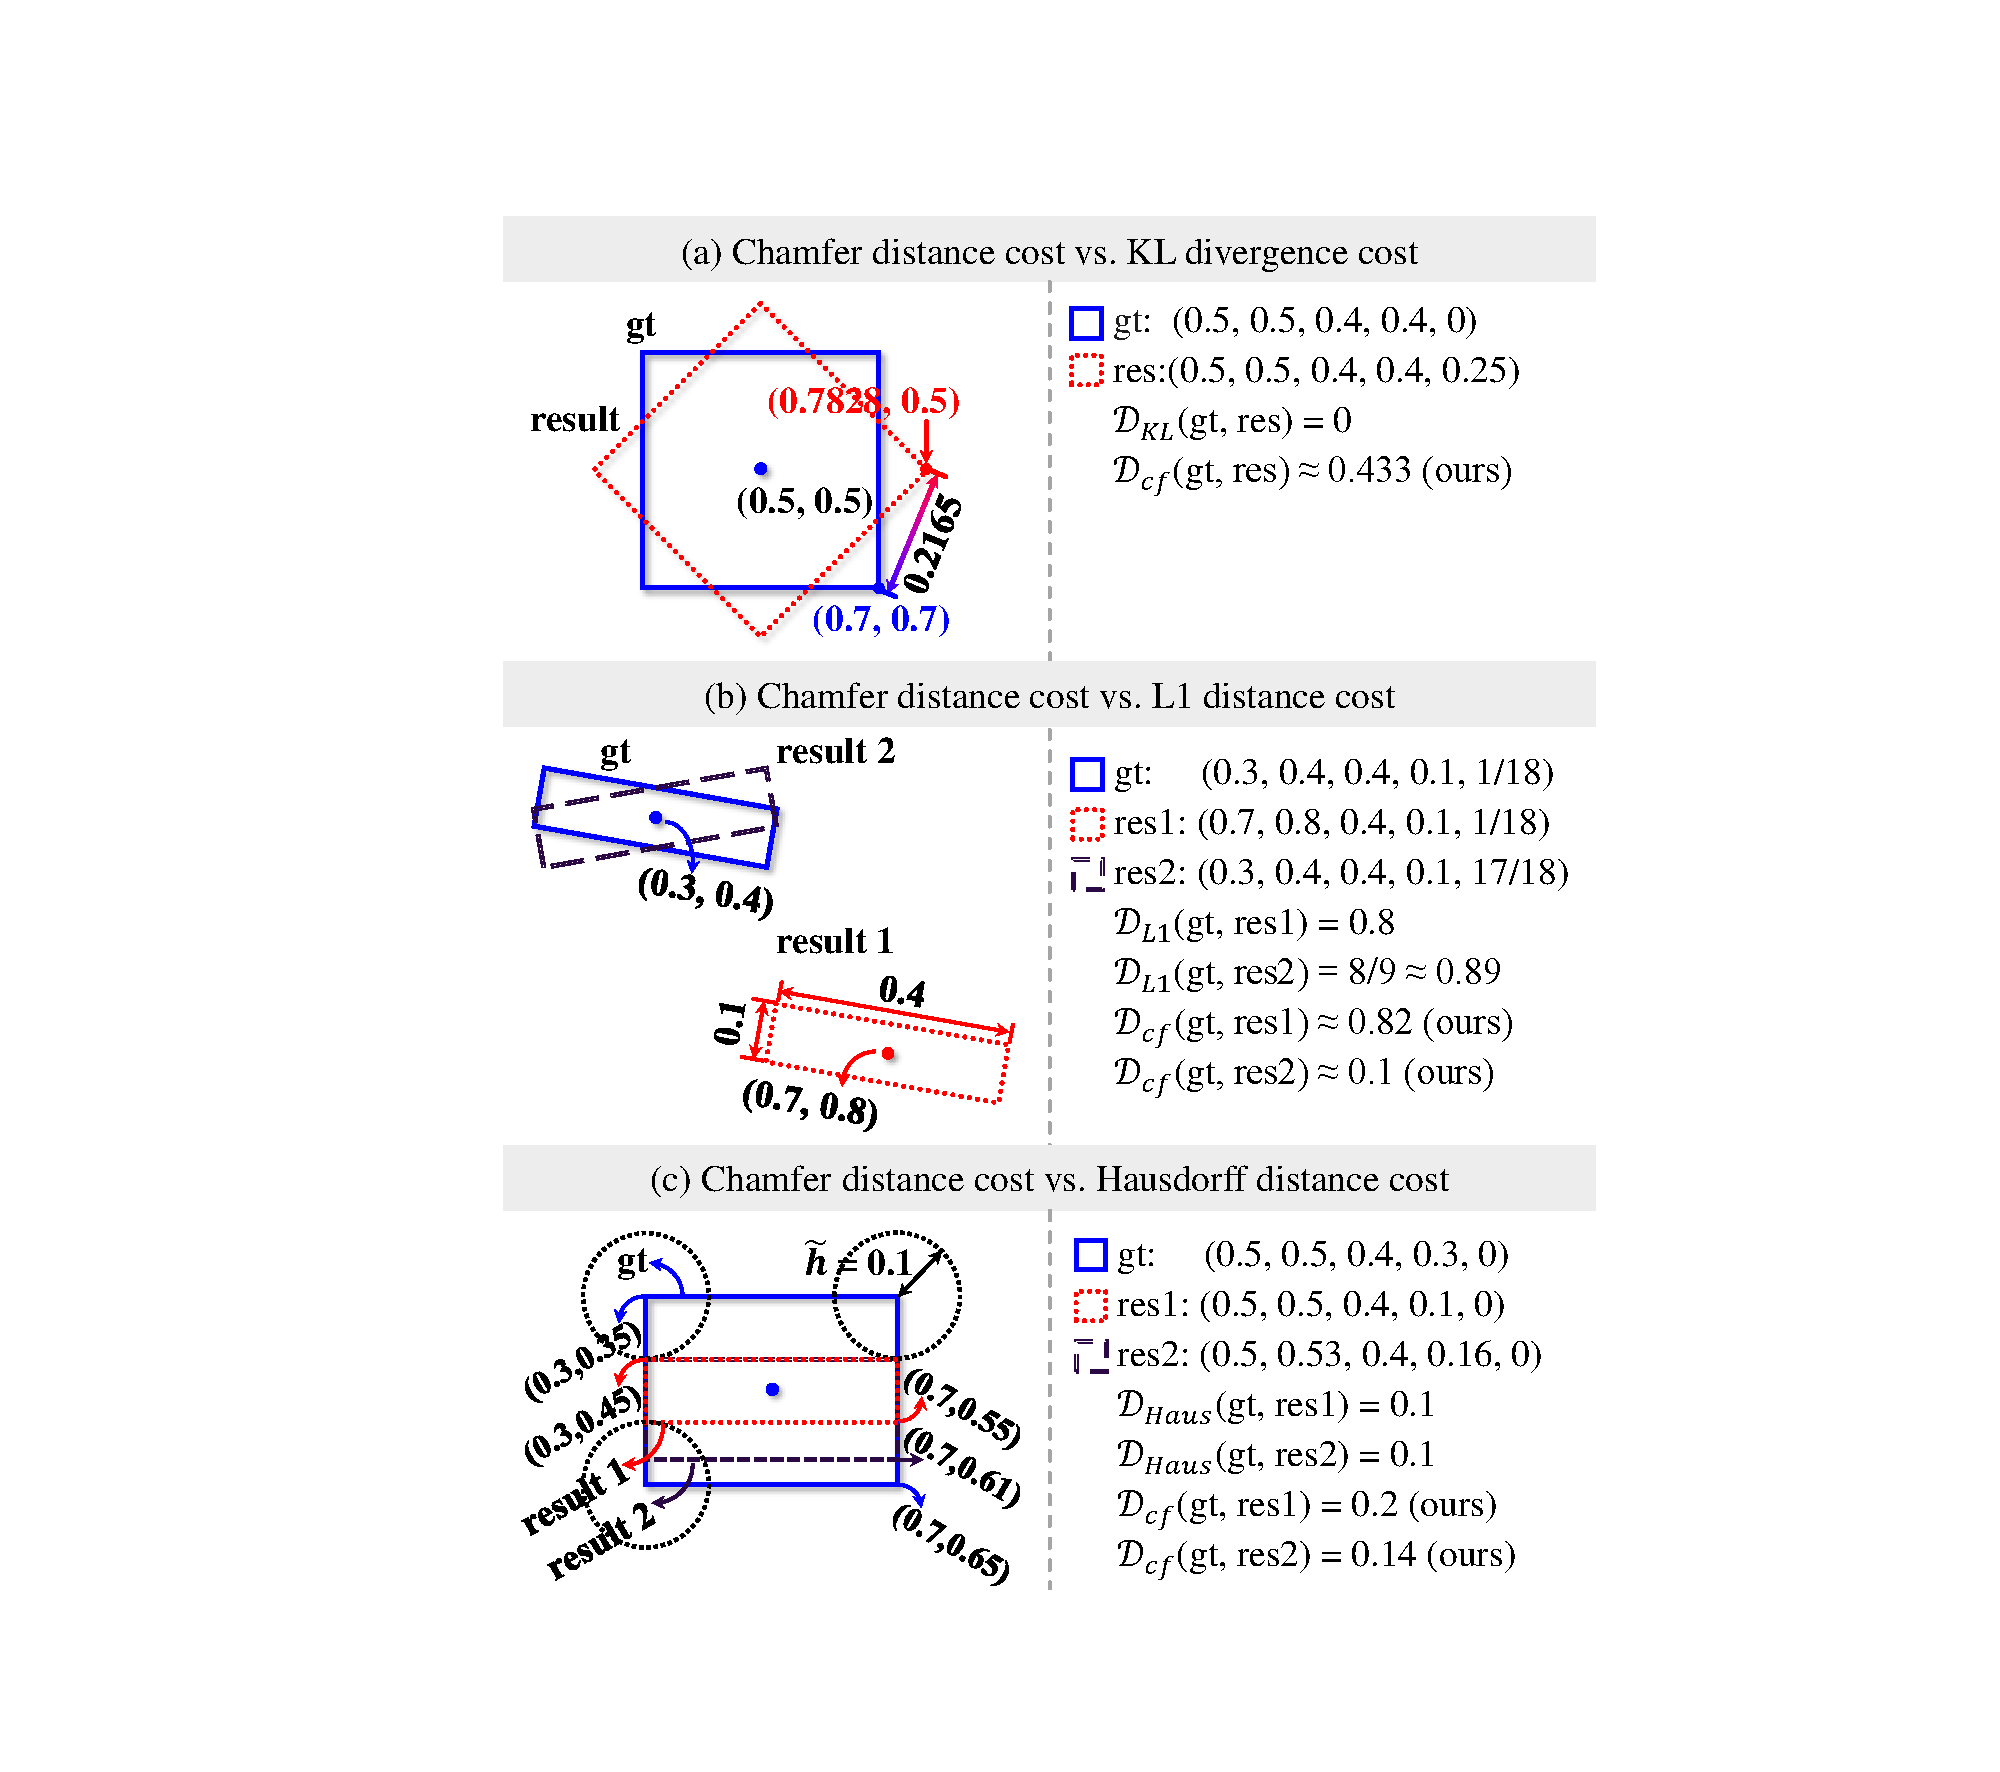
\includegraphics[width=0.95\linewidth]{visual_chamfer.pdf}
  \caption{Comparison of Chamfer distance cost with KL divergence, L1, and Hausdorff distance costs. The centers, sizes, and angles are normalized.}
  \label{visual_chamfer}
  \vspace{-0.5em}
\end{figure}


}


\newcommand{\visualRoatedAttn}{
    \begin{figure}[t]
      \centering
       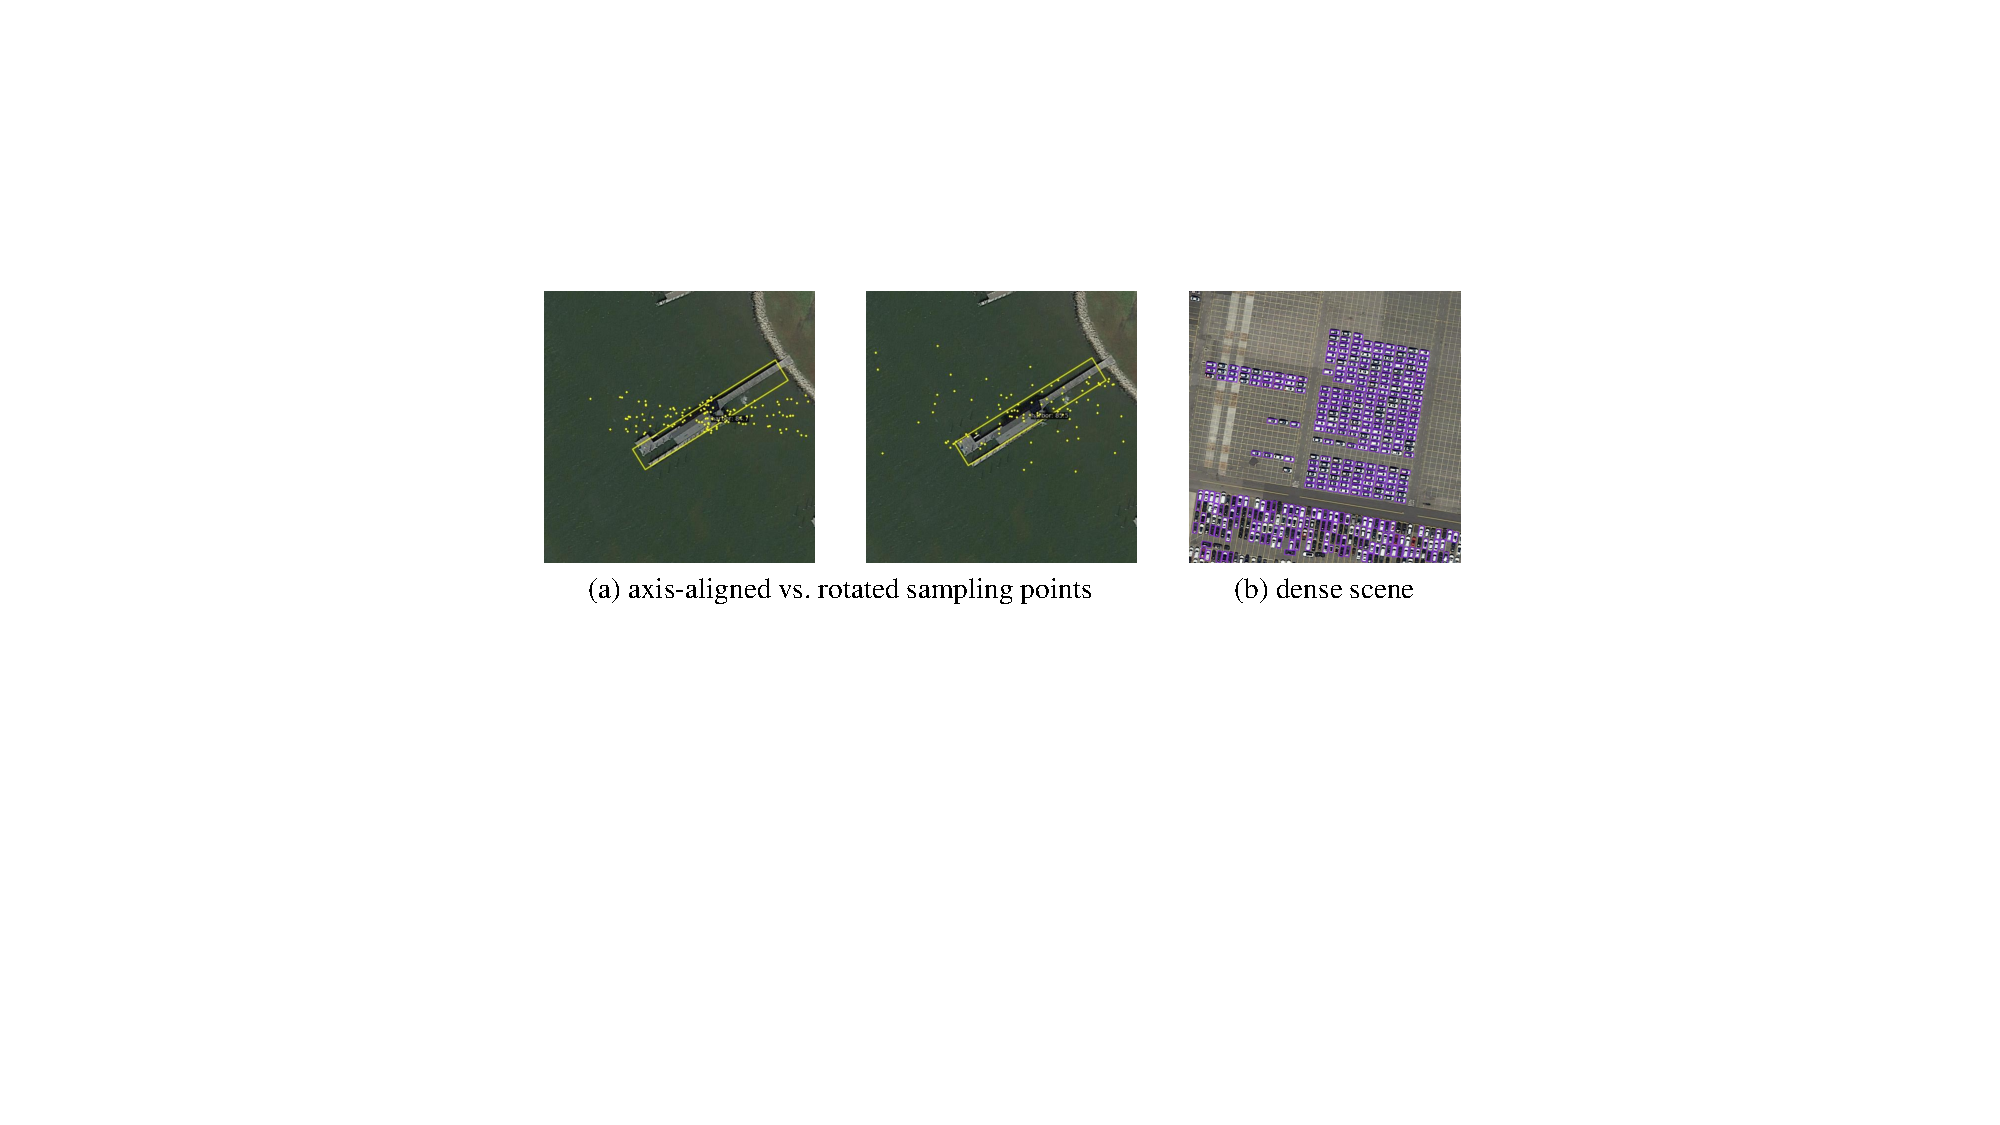
\includegraphics[width=0.95\linewidth]{visual_rotated_attn.pdf}
       \caption{(a) Sampling points in cross attention. $\textcolor[rgb]{1,1,0}{\blacksquare}$ denotes harbors. (b) Suboptimal detection results in dense scenes. $\textcolor[rgb]{0.6, 0.2, 0.8}{\blacksquare}$ denotes cars.}
       \label{visual_rotated_attn}
    \end{figure}
}


\newcommand{\visualAngleDistRefine}{
    \begin{figure*}[t]
      \centering
       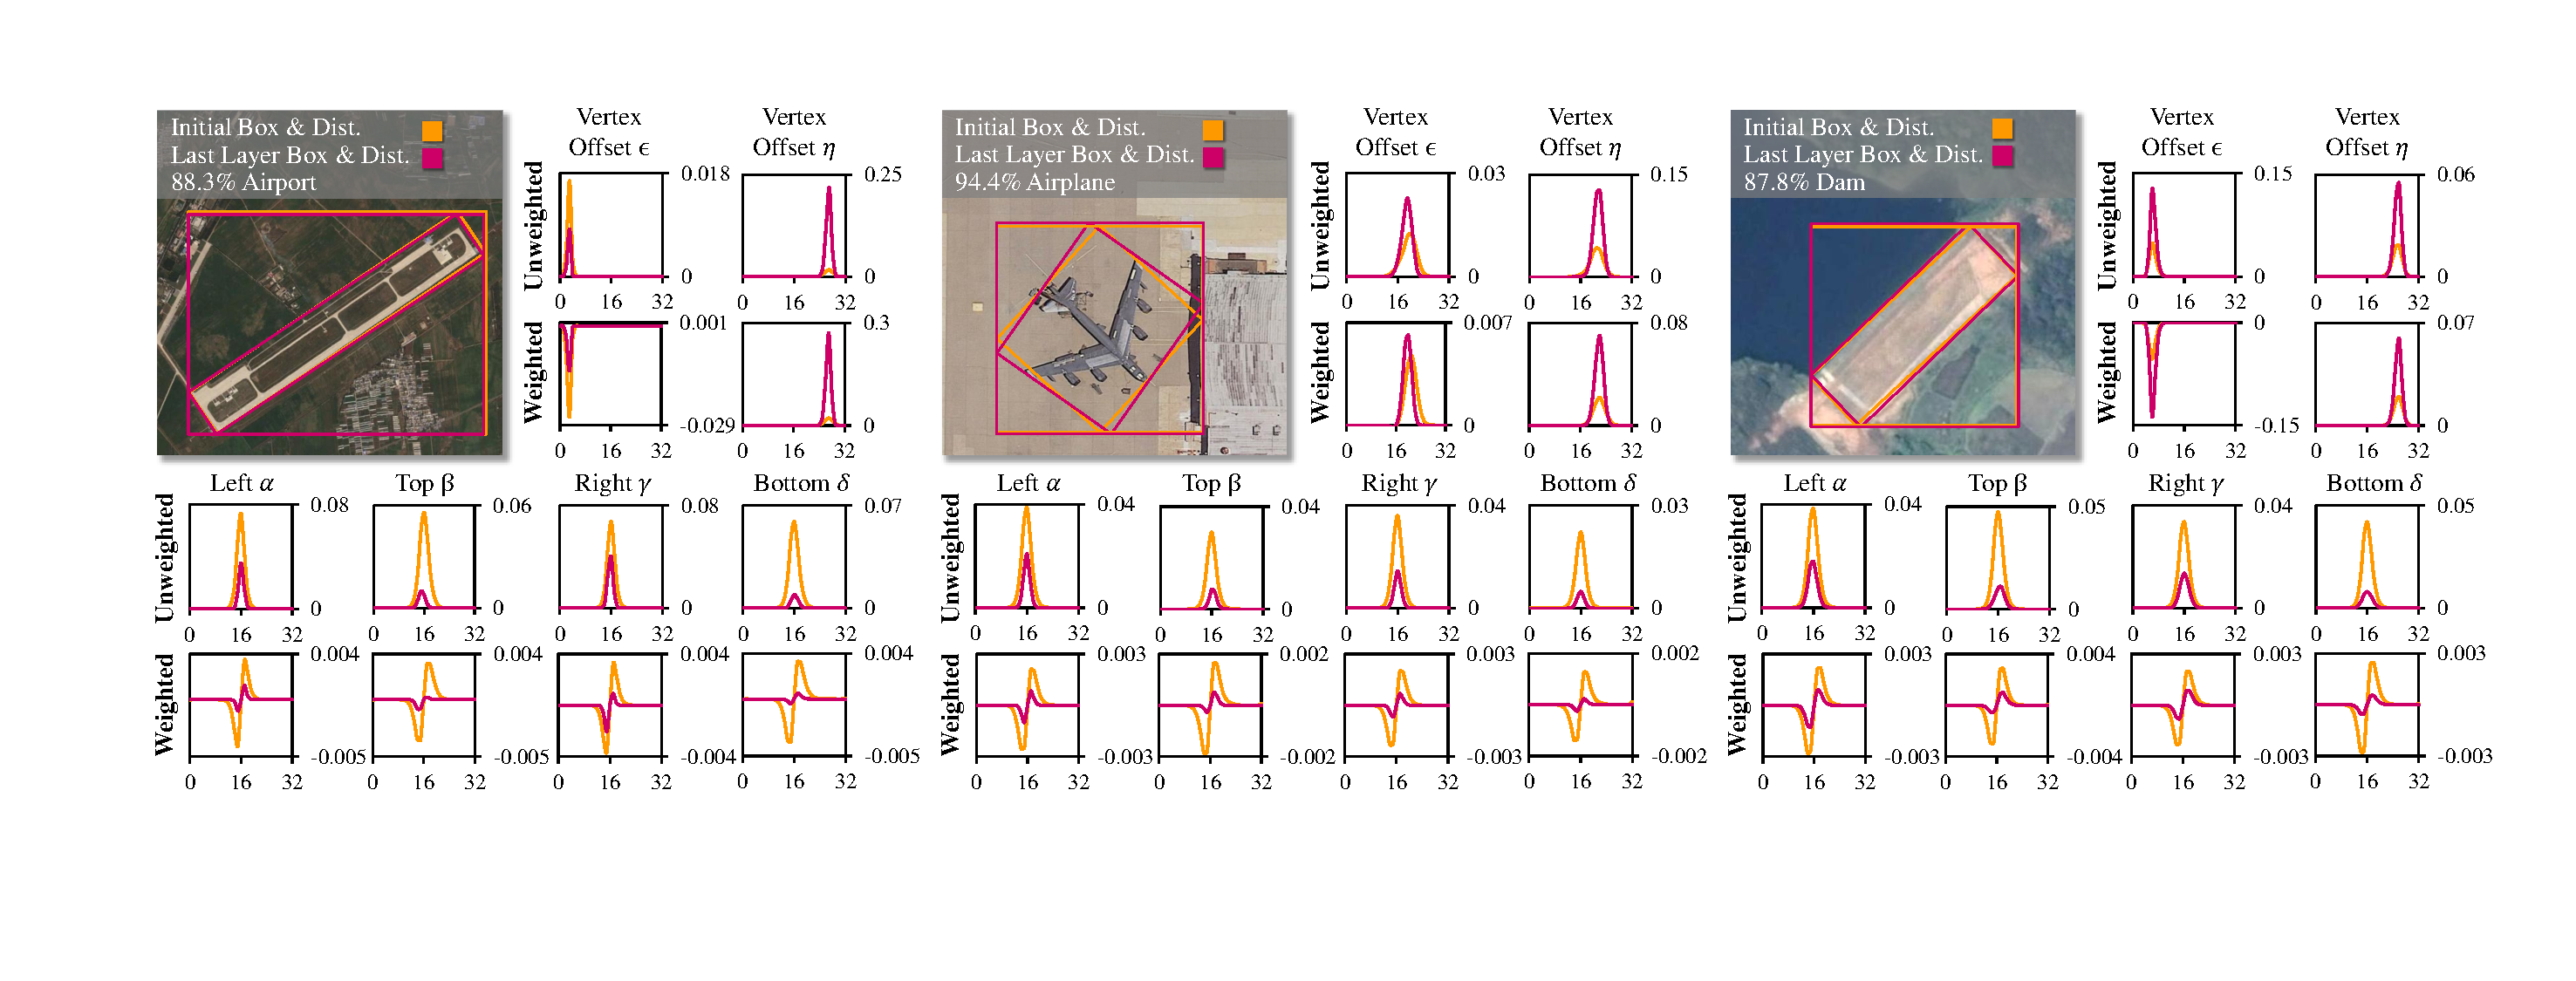
\includegraphics[width=\textwidth]{visual_angle_distribution_refine.pdf}
       \caption{Analysis of Angle Distribution Refinement, including initial and refined oriented boxes, external rectangles, vertex offsets, with unweighted and weighted distributions.}
       \label{visual_angle_dist_refine}
    \end{figure*}
}

\newcommand{\visualresults}{
    \begin{figure*}[t]
      \centering
       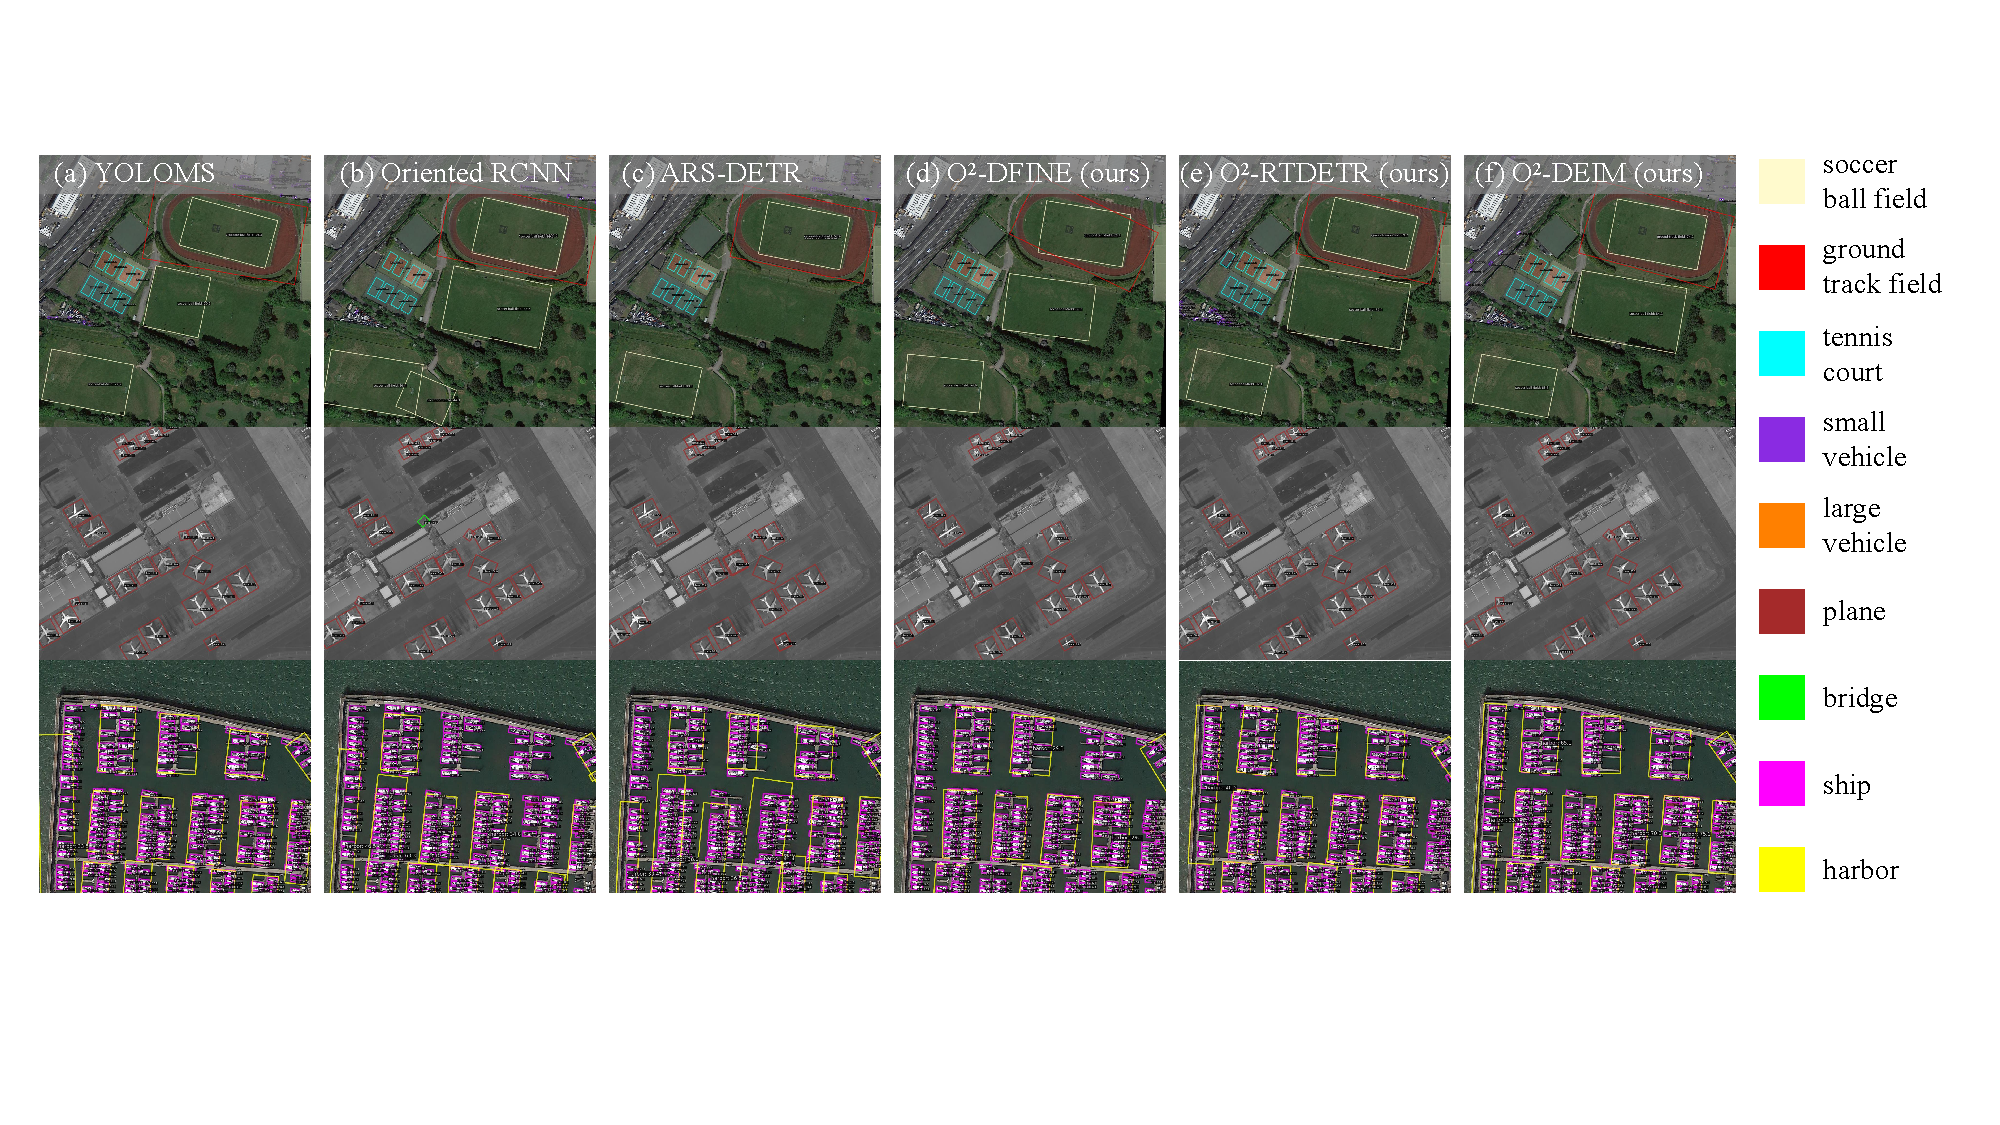
\includegraphics[width=0.95\textwidth]{visual_result_vs_other.pdf}
       \caption{Qualitative comparison between our method and other detectors on challenging scenarios, including large-scale objects (1st row), low-light conditions (2nd row), and densely distributed objects (3rd row). The confidence threshold is set to 0.3}
       \label{visual_results}
    \end{figure*}
}


% appendix

\newcommand{\AppendixvisualRoatedAttn}{
    \begin{figure}[t]
      \centering
       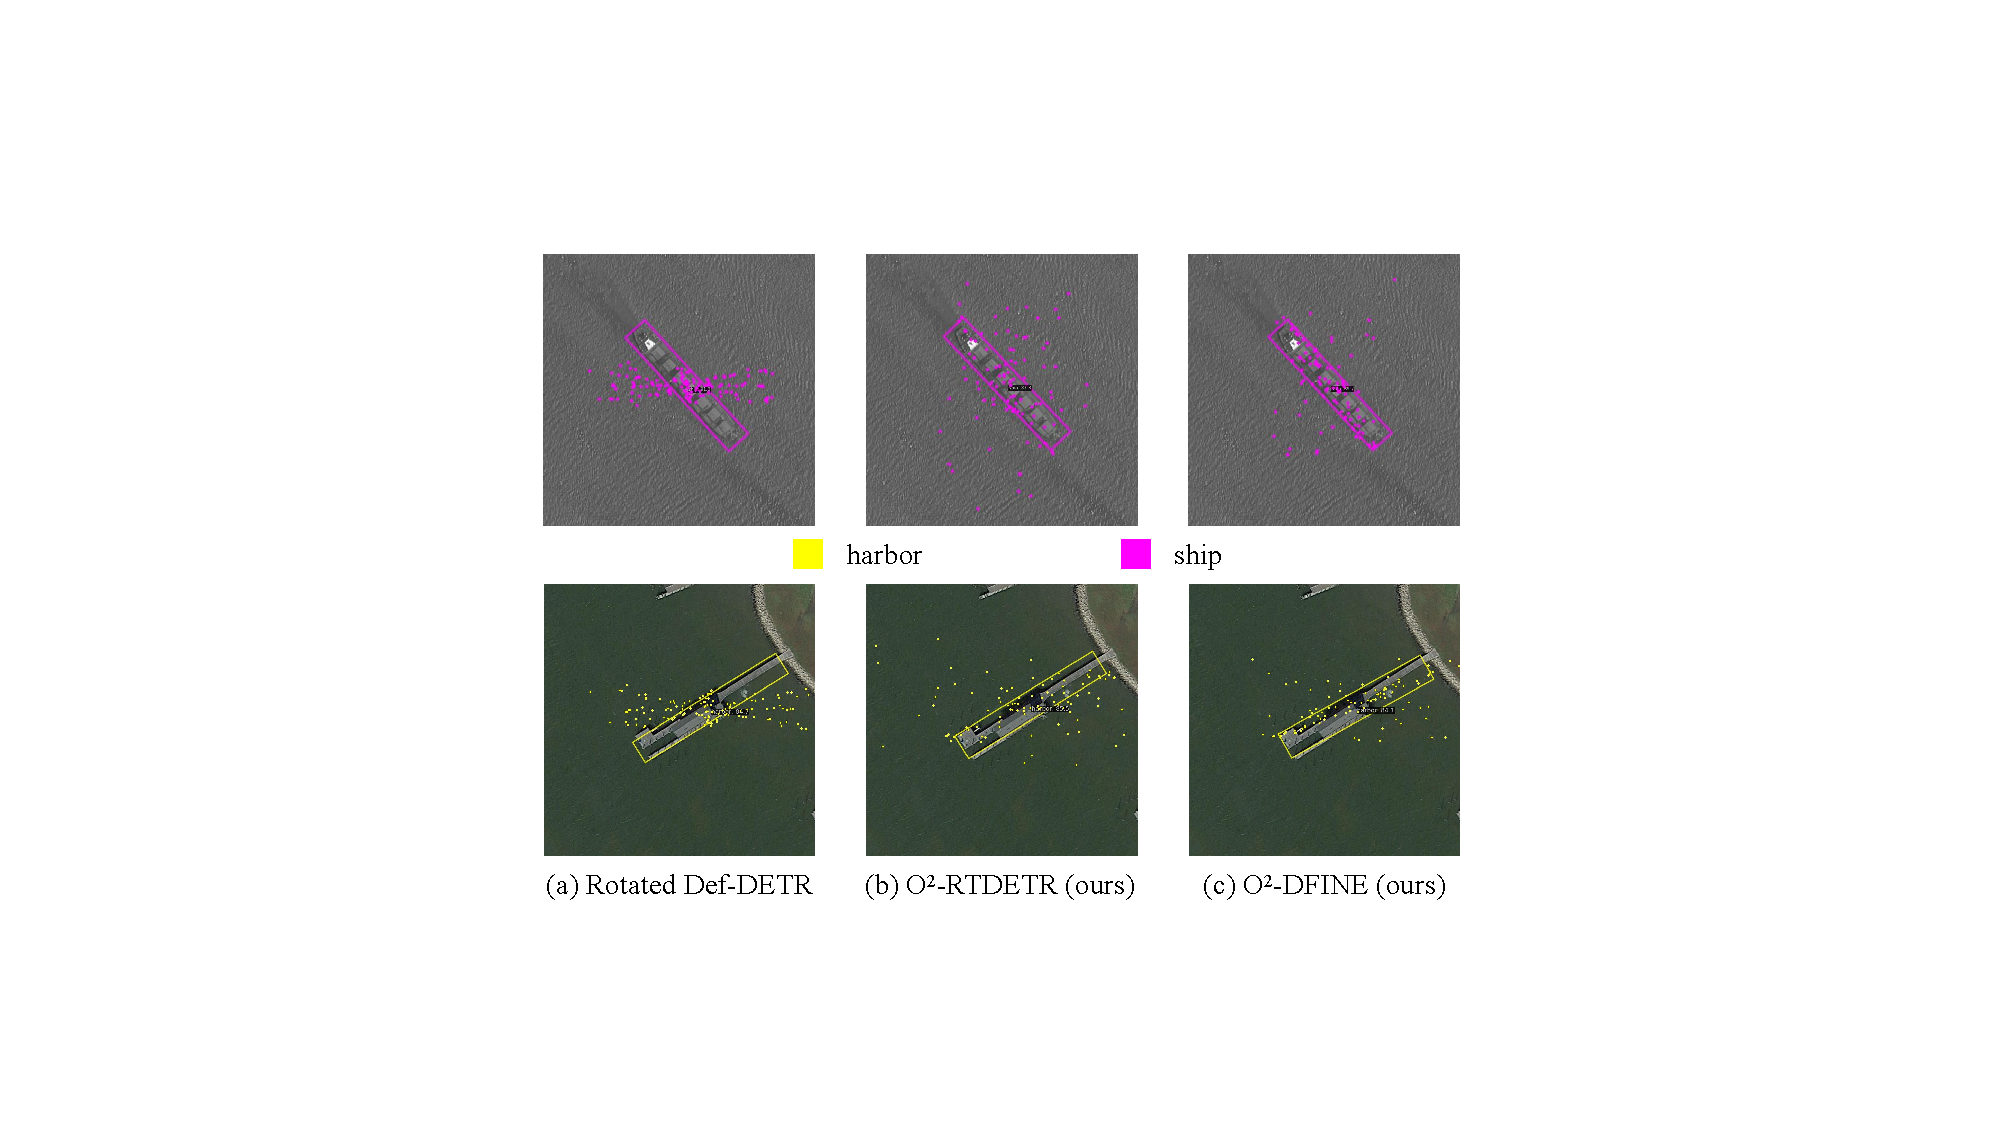
\includegraphics[width=0.95\linewidth]{visual_rotated_attn_appendix.pdf}
       \caption{Visualization of sampling points in cross attention (a) Sampling points in Rotated Deformable DETR. (b) Rotated sampling points in O$^2$-RTDETR. (c) Rotated uneven sampling points in O$^2$-DFINE.}
       \label{appendix_visual_rotated_attn}
    \end{figure}
}
